\section{Methods and data}

\subsection{Data source}
The sequence data is fetched from NCBI protein and nucleotide database, and the transcriptome dataset is fetched from NCBI GEO.

Detailed accession number are listed in Supplementary Material.

\subsection{Multiple sequence alignment}

Multiple sequence alignment is done using Clustal X version 2.1, with default parameters.
Visualization of multiple sequence alignment is done using R package ggmsa \url{https://github.com/YuLab-SMU/ggmsa}. The code is shown in the Supplementary Material.

\subsection{Phylogenetic tree building}
The phylogenetic tree is built using MegaX\upcite{kumar2018mega} Version 10.1.7. The algorithm of building the phylogenetic tree is the Maximum Likelihood algorithm, with parameters shown in the figure below.

\begin{figure}[H]
    \centering
    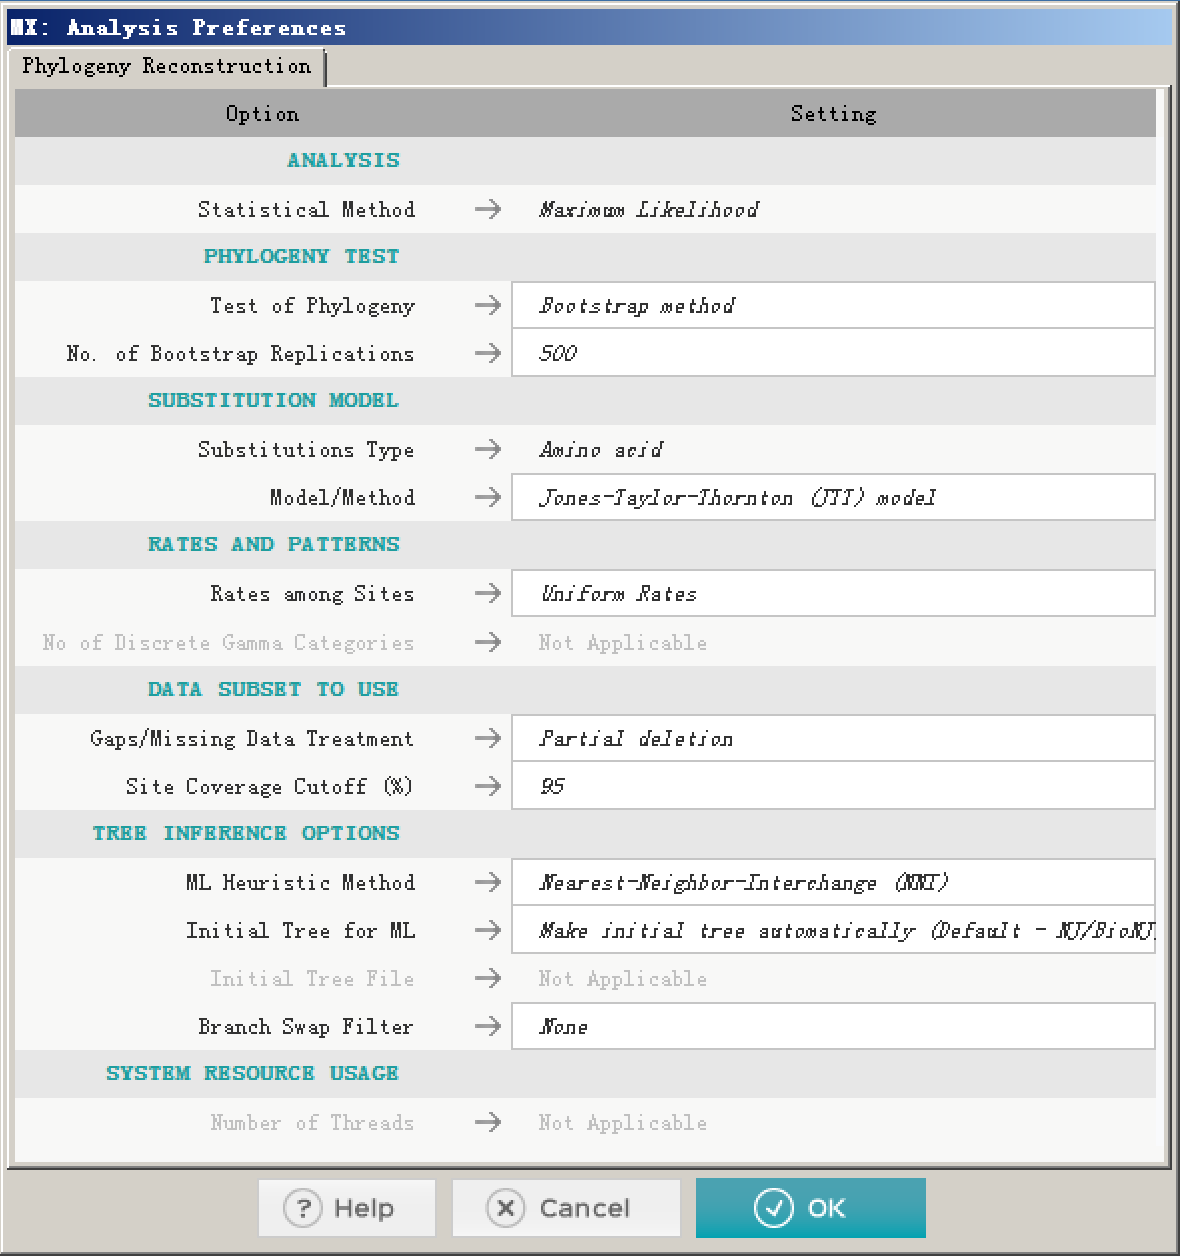
\includegraphics[width=0.5\textwidth]{image/MEGAX.png}
    \caption{Parameters of the phylogenetic tree building}
    \label{MEGAX}
\end{figure}

Then the phylogenetic tree is exported to a \texttt{.nwk} format and used in R for visualization.

\subsection{Protein physicochemical property prediction}
Protein physicochemical property prediction is done using Expasy ProtParam\upcite{gasteiger2005protein}. The complete sequence is analysed.
TMPred\upcite{hofmann1993tmbase} is also used to predict the hydrophobic region of proteins.
\subsection{Nuclear localization signal prediction}
Nuclear localization signal prediction is done using cNLS Mapper\upcite{kosugi2009systematic}, with a cut off set to 2.0.

\subsection{DNA binding site prediction for Cys2His2 zinc finger proteins}
DNA binding site prediction for Cys2His2 zinc finger proteins is done with the Interactive PWM predictor\upcite{persikov2014novo}, and the model used in this tool is expanded linear SVM\upcite{cortes1995support}.

\subsection{Transcriptome analysis}
Transcriptome analysis is done using the code derived from GEO2R. The grouping of the analysis is the same as the grouping in the GSE76510 data series.